%
% Abschlussarbeit mit LaTeX
% ===========================================================================
% This is part of the book "Abschlussarbeit mit LaTeX".
% Copyright (c) 2002-2005 Tobias Erbsland, Andreas Nitsch
% See the file abschlussarbeit_mit_latex.tex for copying conditions.
%

\chapter{Nützliche Pakete}
\index{Pakete}

\section{Anführungszeichen mit dem Paket \enquote{csquotes}}
\index{Anfuehrungszeichen@Anführungszeichen}
\label{sec:anfuehrungszeichen}

Damit Anführungszeichen im gesamten Dokument ein einheitliches Bild abgeben, ist es empfehlenswert das \enquote{csquotes} Paket zu verwenden. Der Vorteil dabei ist, dass durch eine einfache Änderung in der Präambel alle Anführungszeichen im Text geändert werden können. Wenn du, während du an der Abschlussarbeit schreibst, statt die umgangssprachlich genannten Gänsefüßchen neu Guillemets verwenden möchtest, ist das kein grosses Problem. Es reicht, die Optionen des CSQuote Pakets anzupassen und das Dokument durch den \DMLLaTeX"=Kompiler laufen zu lassen.

\subsection{Einbinden des Pakets}

Um das \enquote{csquotes}-Paket zu nutzen bindest du es wie im nachfolgenden Beispiel gezeigt in die die Präambel ein. In den eckigen Klammern wird das Aussehen der Anführungszeichen festgelegt. Gleichzeitig ist es sinnvoll, wenn du dem \enquote{babel}-Paket die Erkennung der Sprache überlässt. Ein ganz einfaches Dokument, welches das beschriebene Paket verwendet könnte so aussehen:

\lstinputlisting[caption={Einfache Anführungszeichen mit dem \enquote{csquotes} Paket},label=lst:csquotes,frame=tb]{listings/csquotes01.tex}

\begin{description}
\item[Zeile 3] Das Paket \enquote{csquote} wird eingebunden. Mit der Option \texttt{german=quotes} werden die deutschen Anführungszeichen '' bzw ,, verwendet.
\item[Zeile 6] Mit dem Kommando \texttt{\textbackslash enquote\{\}} wird der Text zwischen den Klammern in Anführungszeichen gesetzt.
\end{description}

Durch \verb|german=quotes| werden die Anführungszeichen in Form von '' und ,, gesetzt. Weitere Stile für die deutsche Sprache sind Schweizer und franzosische Guillemets ("< und ">). Der Unterschied zwischen den beiden letzteren ist lediglich der Abstand zwischen Anführungszeichen und Text.
\begin{lstlisting}[caption={Häufig verwendete \enquote{csquotes} Optionen.},label=lst:csquotesoptions,frame=tb]
\usepackage[babel,german=quotes]{csquotes} % Deutsche
\usepackage[babel,german=swiss]{csquotes} % Schweizer
\usepackage[babel,german=guillemets]{csquotes} % Französische
\usepackage[babel,english=american]{csquotes} % Amerikanische
\usepackage[babel,english=british]{csquotes} % Englische
\end{lstlisting}

\subsection{Konfigurieren von TeXnicCenter}

Mit dem Befehl \verb|\enquote{| wird der in Anführunsgzeichen stehende Text begonnen und mit einem \verb|}| abgeschlossen. Durch \verb|\enquote{ }| sind auch Verschachtelungen möglich. Diese werden durch das Paket automatisch in Ebenen gegliedert und entsprechende der vorgegebenen Optionen gesetzt. Damit du nicht immer \verb|\enquote{| eintippen musst, solltest du in der Konfiguration von TeXnicCenter zwei Veränderungen vornehmen. Dadurch wird durch Druck auf die Taste "{} vor einem Wort automatisch \verb|\enquote{| gesetzt, respektiv nach einem Wort die abschliessende geschwungene Klammer.

Klicke im Menü auf \enquote{Extras}, dann auf \enquote{Optionen}. Es öffnet sich der Optionen-Dialog (Siehe \cref{fig:konfiguration05}).

\begin{figure}
	\begin{center}
		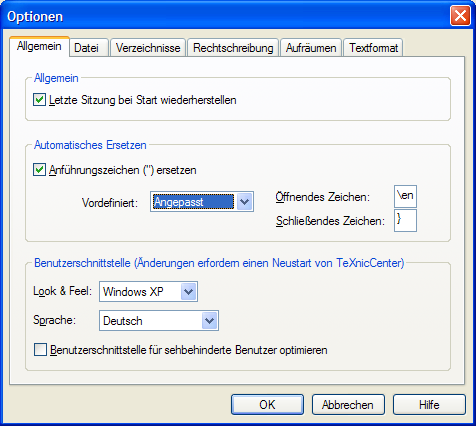
\includegraphics[width=7cm]{images/konfiguration05.png}
		\caption{Konfigurieren der Anführungszeichen}
		\label{fig:konfiguration05}
	\end{center}
\end{figure}

Falls das Kästchen bei \enquote{Anführungszeichen ersetzen} noch nicht markiert ist, markiere es. Danach änderst du im Pull-Down-Menü den Eintrag auf \enquote{Angepasst} sowie den Eintrag bei \enquote{Öffnendes Anführungszeichen} in \texttt{\textbackslash enquote\{} und bei \enquote{Schließendes Anführungszeichen} in \texttt{\}}\footnote{Der Unterschied zwischen den \enquote{Schweizer} und den \foreignquote{french}{Französischen} Anführungszeichen liegt nur im Abstand zwischen Anführungszeichen und Wort. Bei den Schweizer findet sich kein Leerzeichen, bei den Franzosen ein geviert Zwischenraum. Ich verwende in diesem Dokument also die Schweizer, und nicht die Französischen Anführungszeichen.}.

Immer, wenn du jetzt ein einfaches Anführungszeichen (\texttt{''}) eingibst, wird es nun durch ein \textbackslash enquote\{ oder \} ersetzt, je nachdem, ob du dich vor oder hinter einem Wort befindest.

\subsection{Weitere Dokumentation}

Das \enquote{csquotes}-Paket bietet noch eine Fülle an Möglichkeiten, wie zum Beispiel verschiedene Sprachen, Blockquotes und vieles mehr. Die komplette Dokumentation findest du in dem Installationsverzeichniss von MiKTeX unter dem Pfad \enquote{doc\textbackslash latex\textbackslash csquotes}.

